\documentclass[]{article}
\usepackage{lmodern}
\usepackage{amssymb,amsmath}
\usepackage{ifxetex,ifluatex}
\usepackage{fixltx2e} % provides \textsubscript
\ifnum 0\ifxetex 1\fi\ifluatex 1\fi=0 % if pdftex
  \usepackage[T1]{fontenc}
  \usepackage[utf8]{inputenc}
\else % if luatex or xelatex
  \ifxetex
    \usepackage{mathspec}
  \else
    \usepackage{fontspec}
  \fi
  \defaultfontfeatures{Ligatures=TeX,Scale=MatchLowercase}
\fi
% use upquote if available, for straight quotes in verbatim environments
\IfFileExists{upquote.sty}{\usepackage{upquote}}{}
% use microtype if available
\IfFileExists{microtype.sty}{%
\usepackage{microtype}
\UseMicrotypeSet[protrusion]{basicmath} % disable protrusion for tt fonts
}{}
\usepackage[margin=1in]{geometry}
\usepackage{hyperref}
\hypersetup{unicode=true,
            pdftitle={HW2},
            pdfauthor={James Zhao},
            pdfborder={0 0 0},
            breaklinks=true}
\urlstyle{same}  % don't use monospace font for urls
\usepackage{color}
\usepackage{fancyvrb}
\newcommand{\VerbBar}{|}
\newcommand{\VERB}{\Verb[commandchars=\\\{\}]}
\DefineVerbatimEnvironment{Highlighting}{Verbatim}{commandchars=\\\{\}}
% Add ',fontsize=\small' for more characters per line
\usepackage{framed}
\definecolor{shadecolor}{RGB}{248,248,248}
\newenvironment{Shaded}{\begin{snugshade}}{\end{snugshade}}
\newcommand{\KeywordTok}[1]{\textcolor[rgb]{0.13,0.29,0.53}{\textbf{#1}}}
\newcommand{\DataTypeTok}[1]{\textcolor[rgb]{0.13,0.29,0.53}{#1}}
\newcommand{\DecValTok}[1]{\textcolor[rgb]{0.00,0.00,0.81}{#1}}
\newcommand{\BaseNTok}[1]{\textcolor[rgb]{0.00,0.00,0.81}{#1}}
\newcommand{\FloatTok}[1]{\textcolor[rgb]{0.00,0.00,0.81}{#1}}
\newcommand{\ConstantTok}[1]{\textcolor[rgb]{0.00,0.00,0.00}{#1}}
\newcommand{\CharTok}[1]{\textcolor[rgb]{0.31,0.60,0.02}{#1}}
\newcommand{\SpecialCharTok}[1]{\textcolor[rgb]{0.00,0.00,0.00}{#1}}
\newcommand{\StringTok}[1]{\textcolor[rgb]{0.31,0.60,0.02}{#1}}
\newcommand{\VerbatimStringTok}[1]{\textcolor[rgb]{0.31,0.60,0.02}{#1}}
\newcommand{\SpecialStringTok}[1]{\textcolor[rgb]{0.31,0.60,0.02}{#1}}
\newcommand{\ImportTok}[1]{#1}
\newcommand{\CommentTok}[1]{\textcolor[rgb]{0.56,0.35,0.01}{\textit{#1}}}
\newcommand{\DocumentationTok}[1]{\textcolor[rgb]{0.56,0.35,0.01}{\textbf{\textit{#1}}}}
\newcommand{\AnnotationTok}[1]{\textcolor[rgb]{0.56,0.35,0.01}{\textbf{\textit{#1}}}}
\newcommand{\CommentVarTok}[1]{\textcolor[rgb]{0.56,0.35,0.01}{\textbf{\textit{#1}}}}
\newcommand{\OtherTok}[1]{\textcolor[rgb]{0.56,0.35,0.01}{#1}}
\newcommand{\FunctionTok}[1]{\textcolor[rgb]{0.00,0.00,0.00}{#1}}
\newcommand{\VariableTok}[1]{\textcolor[rgb]{0.00,0.00,0.00}{#1}}
\newcommand{\ControlFlowTok}[1]{\textcolor[rgb]{0.13,0.29,0.53}{\textbf{#1}}}
\newcommand{\OperatorTok}[1]{\textcolor[rgb]{0.81,0.36,0.00}{\textbf{#1}}}
\newcommand{\BuiltInTok}[1]{#1}
\newcommand{\ExtensionTok}[1]{#1}
\newcommand{\PreprocessorTok}[1]{\textcolor[rgb]{0.56,0.35,0.01}{\textit{#1}}}
\newcommand{\AttributeTok}[1]{\textcolor[rgb]{0.77,0.63,0.00}{#1}}
\newcommand{\RegionMarkerTok}[1]{#1}
\newcommand{\InformationTok}[1]{\textcolor[rgb]{0.56,0.35,0.01}{\textbf{\textit{#1}}}}
\newcommand{\WarningTok}[1]{\textcolor[rgb]{0.56,0.35,0.01}{\textbf{\textit{#1}}}}
\newcommand{\AlertTok}[1]{\textcolor[rgb]{0.94,0.16,0.16}{#1}}
\newcommand{\ErrorTok}[1]{\textcolor[rgb]{0.64,0.00,0.00}{\textbf{#1}}}
\newcommand{\NormalTok}[1]{#1}
\usepackage{graphicx,grffile}
\makeatletter
\def\maxwidth{\ifdim\Gin@nat@width>\linewidth\linewidth\else\Gin@nat@width\fi}
\def\maxheight{\ifdim\Gin@nat@height>\textheight\textheight\else\Gin@nat@height\fi}
\makeatother
% Scale images if necessary, so that they will not overflow the page
% margins by default, and it is still possible to overwrite the defaults
% using explicit options in \includegraphics[width, height, ...]{}
\setkeys{Gin}{width=\maxwidth,height=\maxheight,keepaspectratio}
\IfFileExists{parskip.sty}{%
\usepackage{parskip}
}{% else
\setlength{\parindent}{0pt}
\setlength{\parskip}{6pt plus 2pt minus 1pt}
}
\setlength{\emergencystretch}{3em}  % prevent overfull lines
\providecommand{\tightlist}{%
  \setlength{\itemsep}{0pt}\setlength{\parskip}{0pt}}
\setcounter{secnumdepth}{0}
% Redefines (sub)paragraphs to behave more like sections
\ifx\paragraph\undefined\else
\let\oldparagraph\paragraph
\renewcommand{\paragraph}[1]{\oldparagraph{#1}\mbox{}}
\fi
\ifx\subparagraph\undefined\else
\let\oldsubparagraph\subparagraph
\renewcommand{\subparagraph}[1]{\oldsubparagraph{#1}\mbox{}}
\fi

%%% Use protect on footnotes to avoid problems with footnotes in titles
\let\rmarkdownfootnote\footnote%
\def\footnote{\protect\rmarkdownfootnote}

%%% Change title format to be more compact
\usepackage{titling}

% Create subtitle command for use in maketitle
\providecommand{\subtitle}[1]{
  \posttitle{
    \begin{center}\large#1\end{center}
    }
}

\setlength{\droptitle}{-2em}

  \title{HW2}
    \pretitle{\vspace{\droptitle}\centering\huge}
  \posttitle{\par}
    \author{James Zhao}
    \preauthor{\centering\large\emph}
  \postauthor{\par}
      \predate{\centering\large\emph}
  \postdate{\par}
    \date{April 24, 2019}


\begin{document}
\maketitle

\section{Q1 Data Collection}\label{q1-data-collection}

\subsection{1.1 Scraping}\label{scraping}

\begin{Shaded}
\begin{Highlighting}[]
\KeywordTok{setwd}\NormalTok{(}\StringTok{"~/GitHub/MMSS_311_2"}\NormalTok{)}
\KeywordTok{library}\NormalTok{(}\StringTok{"xml2"}\NormalTok{)}
\KeywordTok{library}\NormalTok{(}\StringTok{"rvest"}\NormalTok{)}
\KeywordTok{library}\NormalTok{(}\StringTok{"dplyr"}\NormalTok{)}
\end{Highlighting}
\end{Shaded}

\begin{verbatim}
## 
## Attaching package: 'dplyr'
\end{verbatim}

\begin{verbatim}
## The following objects are masked from 'package:stats':
## 
##     filter, lag
\end{verbatim}

\begin{verbatim}
## The following objects are masked from 'package:base':
## 
##     intersect, setdiff, setequal, union
\end{verbatim}

\begin{Shaded}
\begin{Highlighting}[]
\NormalTok{pg <-}\StringTok{ }\KeywordTok{read_html}\NormalTok{(}\StringTok{"https://en.wikipedia.org/wiki/Category:Member_states_of_the_Association_of_Southeast_Asian_Nations"}\NormalTok{)}


\NormalTok{countrytext <-}\StringTok{ }\NormalTok{pg }\OperatorTok
\StringTok{  }\KeywordTok{html_nodes}\NormalTok{(}\StringTok{".mw-category-group+ .mw-category-group a"}\NormalTok{) }\OperatorTok
\StringTok{  }\KeywordTok{html_text}\NormalTok{()}
\NormalTok{countrytext}
\end{Highlighting}
\end{Shaded}

\begin{verbatim}
##  [1] "Brunei"      "Cambodia"    "Indonesia"   "Laos"        "Malaysia"   
##  [6] "Myanmar"     "Philippines" "Singapore"   "Thailand"    "Vietnam"
\end{verbatim}

\begin{Shaded}
\begin{Highlighting}[]
\NormalTok{countryurl <-}\StringTok{ }\NormalTok{pg }\OperatorTok
\StringTok{  }\KeywordTok{html_nodes}\NormalTok{(}\StringTok{".mw-category-group+ .mw-category-group a"}\NormalTok{) }\OperatorTok
\StringTok{  }\KeywordTok{html_attr}\NormalTok{(}\StringTok{"href"}\NormalTok{)}
\NormalTok{countryurl}
\end{Highlighting}
\end{Shaded}

\begin{verbatim}
##  [1] "/wiki/Brunei"      "/wiki/Cambodia"    "/wiki/Indonesia"  
##  [4] "/wiki/Laos"        "/wiki/Malaysia"    "/wiki/Myanmar"    
##  [7] "/wiki/Philippines" "/wiki/Singapore"   "/wiki/Thailand"   
## [10] "/wiki/Vietnam"
\end{verbatim}

\begin{Shaded}
\begin{Highlighting}[]
\NormalTok{data <-}\StringTok{ }\KeywordTok{data.frame}\NormalTok{(}
\NormalTok{  countrytext, countryurl, }
  \DataTypeTok{stringsAsFactors =}\NormalTok{ F) }\OperatorTok
\StringTok{  }\KeywordTok{mutate}\NormalTok{(}\DataTypeTok{countryurl =} \KeywordTok{paste0}\NormalTok{(}\StringTok{"https://en.wikipedia.org"}\NormalTok{, countryurl))}
\KeywordTok{head}\NormalTok{(data)}
\end{Highlighting}
\end{Shaded}

\begin{verbatim}
##   countrytext                              countryurl
## 1      Brunei    https://en.wikipedia.org/wiki/Brunei
## 2    Cambodia  https://en.wikipedia.org/wiki/Cambodia
## 3   Indonesia https://en.wikipedia.org/wiki/Indonesia
## 4        Laos      https://en.wikipedia.org/wiki/Laos
## 5    Malaysia  https://en.wikipedia.org/wiki/Malaysia
## 6     Myanmar   https://en.wikipedia.org/wiki/Myanmar
\end{verbatim}

\begin{Shaded}
\begin{Highlighting}[]
\ControlFlowTok{for}\NormalTok{(i }\ControlFlowTok{in} \DecValTok{1}\OperatorTok{:}\KeywordTok{nrow}\NormalTok{(data)) \{ }
\NormalTok{  data}\OperatorTok{$}\NormalTok{text[i] <-}\StringTok{ }\NormalTok{data}\OperatorTok{$}\NormalTok{countryurl[}\DecValTok{1}\NormalTok{] }\OperatorTok
\StringTok{  }\KeywordTok{read_html}\NormalTok{() }\OperatorTok
\StringTok{  }\KeywordTok{html_nodes}\NormalTok{(}\StringTok{"p"}\NormalTok{) }\OperatorTok
\StringTok{  }\KeywordTok{html_text}\NormalTok{() }\OperatorTok
\StringTok{    }\KeywordTok{paste}\NormalTok{(}\DataTypeTok{collapse =} \StringTok{"}\CharTok{\textbackslash{}n\textbackslash{}n}\StringTok{"}\NormalTok{)}
\NormalTok{\}}
\end{Highlighting}
\end{Shaded}

\section{Q2 Pre-Processing \& Word Frequency
Analysis}\label{q2-pre-processing-word-frequency-analysis}

\subsection{Q2.1 Pre-Process}\label{q2.1-pre-process}

\begin{Shaded}
\begin{Highlighting}[]
\KeywordTok{library}\NormalTok{(tm)}
\end{Highlighting}
\end{Shaded}

\begin{verbatim}
## Loading required package: NLP
\end{verbatim}

\begin{Shaded}
\begin{Highlighting}[]
\NormalTok{tweets <-}\StringTok{ }\KeywordTok{read.csv}\NormalTok{(}\StringTok{"trumptweets.csv"}\NormalTok{)}
\NormalTok{trumptweets <-}\StringTok{ }\KeywordTok{Corpus}\NormalTok{(}\KeywordTok{VectorSource}\NormalTok{(tweets}\OperatorTok{$}\NormalTok{text))}
\NormalTok{trumptweets <-}\StringTok{ }\KeywordTok{tm_map}\NormalTok{(trumptweets, removePunctuation)}
\end{Highlighting}
\end{Shaded}

\begin{verbatim}
## Warning in tm_map.SimpleCorpus(trumptweets, removePunctuation):
## transformation drops documents
\end{verbatim}

\begin{Shaded}
\begin{Highlighting}[]
\NormalTok{trumptweets <-}\StringTok{ }\KeywordTok{tm_map}\NormalTok{(trumptweets, tolower)}
\end{Highlighting}
\end{Shaded}

\begin{verbatim}
## Warning in tm_map.SimpleCorpus(trumptweets, tolower): transformation drops
## documents
\end{verbatim}

\begin{Shaded}
\begin{Highlighting}[]
\NormalTok{trumptweets <-}\StringTok{ }\KeywordTok{tm_map}\NormalTok{(trumptweets, removeWords, }\KeywordTok{stopwords}\NormalTok{(}\StringTok{"en"}\NormalTok{))}
\end{Highlighting}
\end{Shaded}

\begin{verbatim}
## Warning in tm_map.SimpleCorpus(trumptweets, removeWords, stopwords("en")):
## transformation drops documents
\end{verbatim}

\begin{Shaded}
\begin{Highlighting}[]
\NormalTok{trumptweets <-}\StringTok{ }\KeywordTok{tm_map}\NormalTok{(trumptweets,stemDocument)}
\end{Highlighting}
\end{Shaded}

\begin{verbatim}
## Warning in tm_map.SimpleCorpus(trumptweets, stemDocument): transformation
## drops documents
\end{verbatim}

\begin{Shaded}
\begin{Highlighting}[]
\NormalTok{dtm <-}\StringTok{ }\KeywordTok{DocumentTermMatrix}\NormalTok{(trumptweets)}
\NormalTok{dtm <-}\StringTok{ }\KeywordTok{removeSparseTerms}\NormalTok{(dtm,.}\DecValTok{99}\NormalTok{)}

\KeywordTok{library}\NormalTok{(}\StringTok{"tidyverse"}\NormalTok{)}
\end{Highlighting}
\end{Shaded}

\begin{verbatim}
## -- Attaching packages ---------------------------------------------------------------- tidyverse 1.2.1 --
\end{verbatim}

\begin{verbatim}
## v ggplot2 3.1.1     v readr   1.3.1
## v tibble  2.1.1     v purrr   0.3.2
## v tidyr   0.8.3     v stringr 1.4.0
## v ggplot2 3.1.1     v forcats 0.4.0
\end{verbatim}

\begin{verbatim}
## -- Conflicts ------------------------------------------------------------------- tidyverse_conflicts() --
## x ggplot2::annotate()     masks NLP::annotate()
## x dplyr::filter()         masks stats::filter()
## x readr::guess_encoding() masks rvest::guess_encoding()
## x dplyr::lag()            masks stats::lag()
## x purrr::pluck()          masks rvest::pluck()
\end{verbatim}

\begin{Shaded}
\begin{Highlighting}[]
\KeywordTok{library}\NormalTok{(}\StringTok{"tidytext"}\NormalTok{)}
\NormalTok{tidy_dtm <-}\StringTok{ }\KeywordTok{tidy}\NormalTok{(dtm)}
\NormalTok{dtm.mat <-}\StringTok{ }\KeywordTok{as.matrix}\NormalTok{(dtm)}

\NormalTok{dtm_tfidf <-}\StringTok{ }\KeywordTok{DocumentTermMatrix}\NormalTok{(trumptweets, }\DataTypeTok{control =} \KeywordTok{list}\NormalTok{(}\DataTypeTok{weighting =}\NormalTok{ weightTfIdf))}
\end{Highlighting}
\end{Shaded}

\begin{verbatim}
## Warning in weighting(x): empty document(s): 2003 20135
\end{verbatim}

\subsection{Q2.2 Word Frequency/Dictionary
Methods}\label{q2.2-word-frequencydictionary-methods}

\subsubsection{(a)}\label{a}

\begin{Shaded}
\begin{Highlighting}[]
\NormalTok{tidy_dtm }\OperatorTok\StringTok{ }\KeywordTok{group_by}\NormalTok{(term) }\OperatorTok
\StringTok{  }\KeywordTok{summarize}\NormalTok{(}\DataTypeTok{freq =} \KeywordTok{sum}\NormalTok{(count)) }\OperatorTok
\StringTok{  }\KeywordTok{top_n}\NormalTok{(}\DecValTok{20}\NormalTok{, freq) }\OperatorTok
\StringTok{  }\KeywordTok{arrange}\NormalTok{(}\KeywordTok{desc}\NormalTok{(freq))}
\end{Highlighting}
\end{Shaded}

\begin{verbatim}
## # A tibble: 20 x 2
##    term             freq
##    <chr>           <dbl>
##  1 realdonaldtrump  8469
##  2 trump            4359
##  3 great            4266
##  4 will             4232
##  5 thank            3974
##  6 twitter          2868
##  7 amp              2725
##  8 presid           2019
##  9 just             1773
## 10 get              1704
## 11 make             1549
## 12 peopl            1495
## 13 donald           1488
## 14 obama            1367
## 15 america          1363
## 16 run              1335
## 17 like             1321
## 18 need             1298
## 19 time             1289
## 20 new              1282
\end{verbatim}

\begin{Shaded}
\begin{Highlighting}[]
\NormalTok{tidy_dtm }\OperatorTok\StringTok{ }\KeywordTok{group_by}\NormalTok{(term) }\OperatorTok
\StringTok{  }\KeywordTok{summarize}\NormalTok{(}\DataTypeTok{freq =} \KeywordTok{sum}\NormalTok{(count)) }\OperatorTok
\StringTok{  }\KeywordTok{top_n}\NormalTok{(}\DecValTok{20}\NormalTok{, freq) }\OperatorTok
\StringTok{  }\KeywordTok{arrange}\NormalTok{(}\KeywordTok{desc}\NormalTok{(freq)) }\OperatorTok
\StringTok{  }\KeywordTok{ggplot}\NormalTok{(}\KeywordTok{aes}\NormalTok{(}\KeywordTok{reorder}\NormalTok{(term, }\OperatorTok{-}\NormalTok{freq), freq)) }\OperatorTok{+}
\StringTok{  }\KeywordTok{geom_bar}\NormalTok{(}\DataTypeTok{stat=}\StringTok{"identity"}\NormalTok{) }\OperatorTok{+}
\StringTok{  }\KeywordTok{theme}\NormalTok{(}\DataTypeTok{axis.text.x =} \KeywordTok{element_text}\NormalTok{(}\DataTypeTok{angle=}\DecValTok{45}\NormalTok{, }\DataTypeTok{hjust=}\DecValTok{1}\NormalTok{)) }\OperatorTok{+}
\StringTok{  }\KeywordTok{xlab}\NormalTok{(}\StringTok{"word"}\NormalTok{)}
\end{Highlighting}
\end{Shaded}

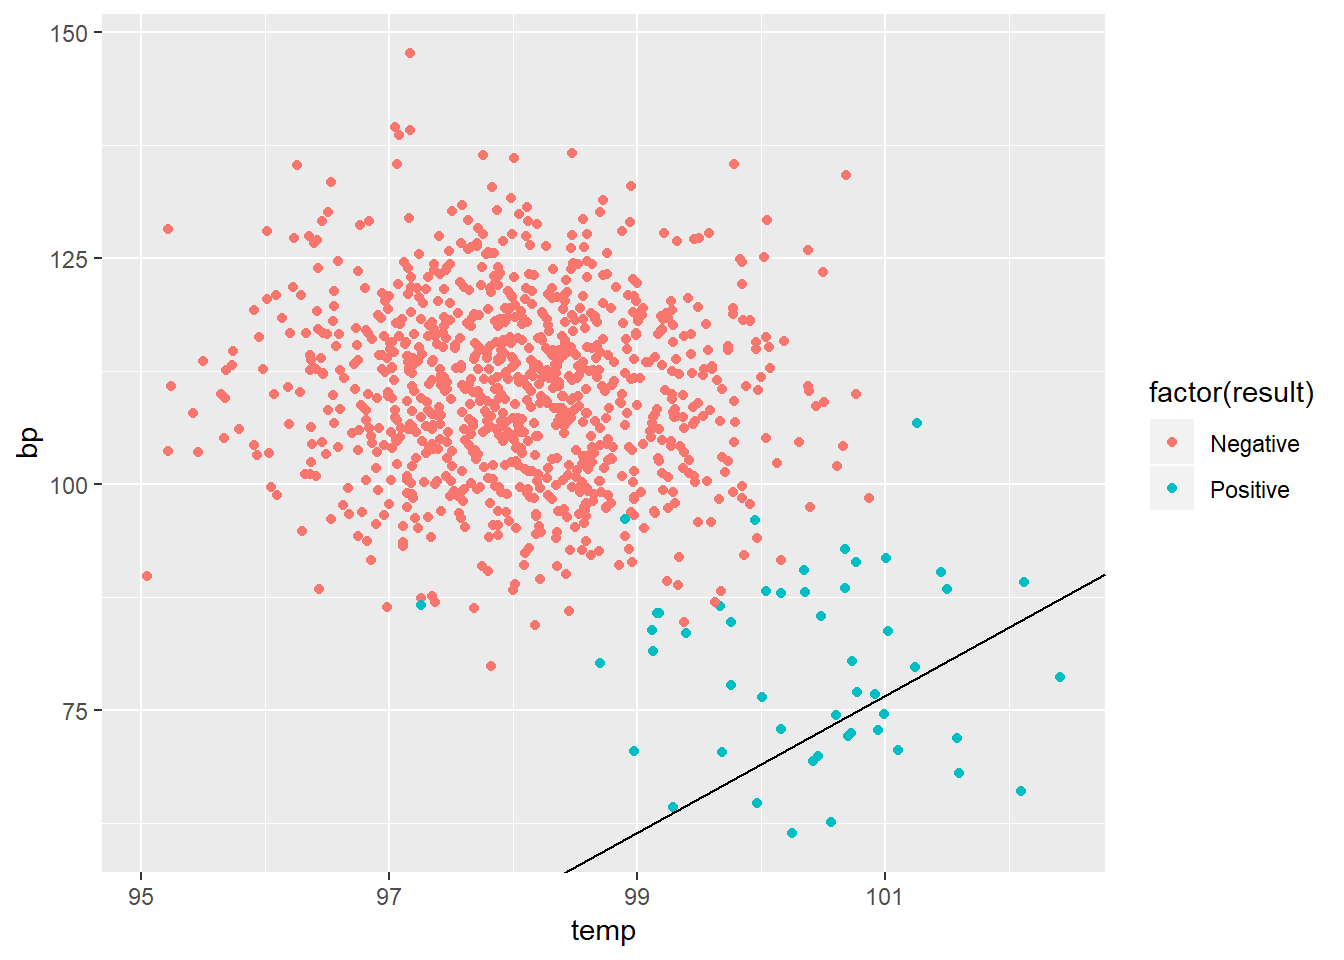
\includegraphics{HW2_files/figure-latex/unnamed-chunk-3-1.pdf}

\subsubsection{(b)}\label{b}

\begin{Shaded}
\begin{Highlighting}[]
\KeywordTok{library}\NormalTok{(lubridate)}
\end{Highlighting}
\end{Shaded}

\begin{verbatim}
## 
## Attaching package: 'lubridate'
\end{verbatim}

\begin{verbatim}
## The following object is masked from 'package:base':
## 
##     date
\end{verbatim}

\begin{Shaded}
\begin{Highlighting}[]
\NormalTok{tweets <-}\StringTok{ }\KeywordTok{mutate}\NormalTok{(tweets, }\DataTypeTok{created_at =} \KeywordTok{mdy_hm}\NormalTok{(created_at))}
\NormalTok{tweets_post <-}\StringTok{ }\KeywordTok{filter}\NormalTok{(tweets, created_at }\OperatorTok{>=}\StringTok{ }\KeywordTok{as.Date}\NormalTok{(}\StringTok{"2016-12-08"}\NormalTok{))}
\NormalTok{tweets_pre <-}\StringTok{ }\KeywordTok{filter}\NormalTok{(tweets, created_at }\OperatorTok{<}\StringTok{ }\KeywordTok{as.Date}\NormalTok{(}\StringTok{"2016-12-08"}\NormalTok{))}

\NormalTok{trumptweets_pre <-}\StringTok{ }\KeywordTok{Corpus}\NormalTok{(}\KeywordTok{VectorSource}\NormalTok{(tweets_pre}\OperatorTok{$}\NormalTok{text))}
\NormalTok{trumptweets_pre <-}\StringTok{ }\KeywordTok{tm_map}\NormalTok{(trumptweets_pre, removePunctuation)}
\end{Highlighting}
\end{Shaded}

\begin{verbatim}
## Warning in tm_map.SimpleCorpus(trumptweets_pre, removePunctuation):
## transformation drops documents
\end{verbatim}

\begin{Shaded}
\begin{Highlighting}[]
\NormalTok{trumptweets_pre <-}\StringTok{ }\KeywordTok{tm_map}\NormalTok{(trumptweets_pre, tolower)}
\end{Highlighting}
\end{Shaded}

\begin{verbatim}
## Warning in tm_map.SimpleCorpus(trumptweets_pre, tolower): transformation
## drops documents
\end{verbatim}

\begin{Shaded}
\begin{Highlighting}[]
\NormalTok{trumptweets_pre <-}\StringTok{ }\KeywordTok{tm_map}\NormalTok{(trumptweets_pre, removeWords, }\KeywordTok{stopwords}\NormalTok{(}\StringTok{"en"}\NormalTok{))}
\end{Highlighting}
\end{Shaded}

\begin{verbatim}
## Warning in tm_map.SimpleCorpus(trumptweets_pre, removeWords,
## stopwords("en")): transformation drops documents
\end{verbatim}

\begin{Shaded}
\begin{Highlighting}[]
\NormalTok{trumptweets_pre <-}\StringTok{ }\KeywordTok{tm_map}\NormalTok{(trumptweets_pre,stemDocument)}
\end{Highlighting}
\end{Shaded}

\begin{verbatim}
## Warning in tm_map.SimpleCorpus(trumptweets_pre, stemDocument):
## transformation drops documents
\end{verbatim}

\begin{Shaded}
\begin{Highlighting}[]
\NormalTok{dtm_pre <-}\StringTok{ }\KeywordTok{DocumentTermMatrix}\NormalTok{(trumptweets_pre)}
\NormalTok{dtm_pre <-}\StringTok{ }\KeywordTok{removeSparseTerms}\NormalTok{(dtm_pre,.}\DecValTok{99}\NormalTok{)}
\NormalTok{tidy_dtm_pre <-}\StringTok{ }\KeywordTok{tidy}\NormalTok{(dtm_pre)}

\NormalTok{trumptweets_post <-}\StringTok{ }\KeywordTok{Corpus}\NormalTok{(}\KeywordTok{VectorSource}\NormalTok{(tweets_post}\OperatorTok{$}\NormalTok{text))}
\NormalTok{trumptweets_post <-}\StringTok{ }\KeywordTok{tm_map}\NormalTok{(trumptweets_post, removePunctuation)}
\end{Highlighting}
\end{Shaded}

\begin{verbatim}
## Warning in tm_map.SimpleCorpus(trumptweets_post, removePunctuation):
## transformation drops documents
\end{verbatim}

\begin{Shaded}
\begin{Highlighting}[]
\NormalTok{trumptweets_post <-}\StringTok{ }\KeywordTok{tm_map}\NormalTok{(trumptweets_post, tolower)}
\end{Highlighting}
\end{Shaded}

\begin{verbatim}
## Warning in tm_map.SimpleCorpus(trumptweets_post, tolower): transformation
## drops documents
\end{verbatim}

\begin{Shaded}
\begin{Highlighting}[]
\NormalTok{trumptweets_post <-}\StringTok{ }\KeywordTok{tm_map}\NormalTok{(trumptweets_post, removeWords, }\KeywordTok{stopwords}\NormalTok{(}\StringTok{"en"}\NormalTok{))}
\end{Highlighting}
\end{Shaded}

\begin{verbatim}
## Warning in tm_map.SimpleCorpus(trumptweets_post, removeWords,
## stopwords("en")): transformation drops documents
\end{verbatim}

\begin{Shaded}
\begin{Highlighting}[]
\NormalTok{trumptweets_post <-}\StringTok{ }\KeywordTok{tm_map}\NormalTok{(trumptweets_post,stemDocument)}
\end{Highlighting}
\end{Shaded}

\begin{verbatim}
## Warning in tm_map.SimpleCorpus(trumptweets_post, stemDocument):
## transformation drops documents
\end{verbatim}

\begin{Shaded}
\begin{Highlighting}[]
\NormalTok{dtm_post <-}\StringTok{ }\KeywordTok{DocumentTermMatrix}\NormalTok{(trumptweets_post)}
\NormalTok{dtm_post <-}\StringTok{ }\KeywordTok{removeSparseTerms}\NormalTok{(dtm_post,.}\DecValTok{99}\NormalTok{)}
\NormalTok{tidy_dtm_post <-}\StringTok{ }\KeywordTok{tidy}\NormalTok{(dtm_post)}

\NormalTok{tidy_dtm_pre }\OperatorTok\StringTok{ }\KeywordTok{group_by}\NormalTok{(term) }\OperatorTok
\StringTok{  }\KeywordTok{summarize}\NormalTok{(}\DataTypeTok{freq =} \KeywordTok{sum}\NormalTok{(count)) }\OperatorTok
\StringTok{  }\KeywordTok{top_n}\NormalTok{(}\DecValTok{20}\NormalTok{, freq) }\OperatorTok
\StringTok{  }\KeywordTok{arrange}\NormalTok{(}\KeywordTok{desc}\NormalTok{(freq))}
\end{Highlighting}
\end{Shaded}

\begin{verbatim}
## # A tibble: 20 x 2
##    term             freq
##    <chr>           <dbl>
##  1 realdonaldtrump  8376
##  2 trump            4199
##  3 thank            3752
##  4 great            3702
##  5 will             3656
##  6 twitter          2861
##  7 amp              2228
##  8 presid           1840
##  9 just             1582
## 10 get              1537
## 11 donald           1464
## 12 make             1398
## 13 obama            1305
## 14 run              1304
## 15 peopl            1264
## 16 like             1251
## 17 need             1216
## 18 america          1179
## 19 new              1167
## 20 can              1161
\end{verbatim}

\begin{Shaded}
\begin{Highlighting}[]
\NormalTok{tidy_dtm_pre }\OperatorTok\StringTok{ }\KeywordTok{group_by}\NormalTok{(term) }\OperatorTok
\StringTok{  }\KeywordTok{summarize}\NormalTok{(}\DataTypeTok{freq =} \KeywordTok{sum}\NormalTok{(count)) }\OperatorTok
\StringTok{  }\KeywordTok{top_n}\NormalTok{(}\DecValTok{20}\NormalTok{, freq) }\OperatorTok
\StringTok{  }\KeywordTok{arrange}\NormalTok{(}\KeywordTok{desc}\NormalTok{(freq)) }\OperatorTok
\StringTok{  }\KeywordTok{ggplot}\NormalTok{(}\KeywordTok{aes}\NormalTok{(}\KeywordTok{reorder}\NormalTok{(term, }\OperatorTok{-}\NormalTok{freq), freq)) }\OperatorTok{+}
\StringTok{  }\KeywordTok{geom_bar}\NormalTok{(}\DataTypeTok{stat=}\StringTok{"identity"}\NormalTok{) }\OperatorTok{+}
\StringTok{  }\KeywordTok{theme}\NormalTok{(}\DataTypeTok{axis.text.x =} \KeywordTok{element_text}\NormalTok{(}\DataTypeTok{angle=}\DecValTok{45}\NormalTok{, }\DataTypeTok{hjust=}\DecValTok{1}\NormalTok{)) }\OperatorTok{+}
\StringTok{  }\KeywordTok{xlab}\NormalTok{(}\StringTok{"word"}\NormalTok{)}
\end{Highlighting}
\end{Shaded}

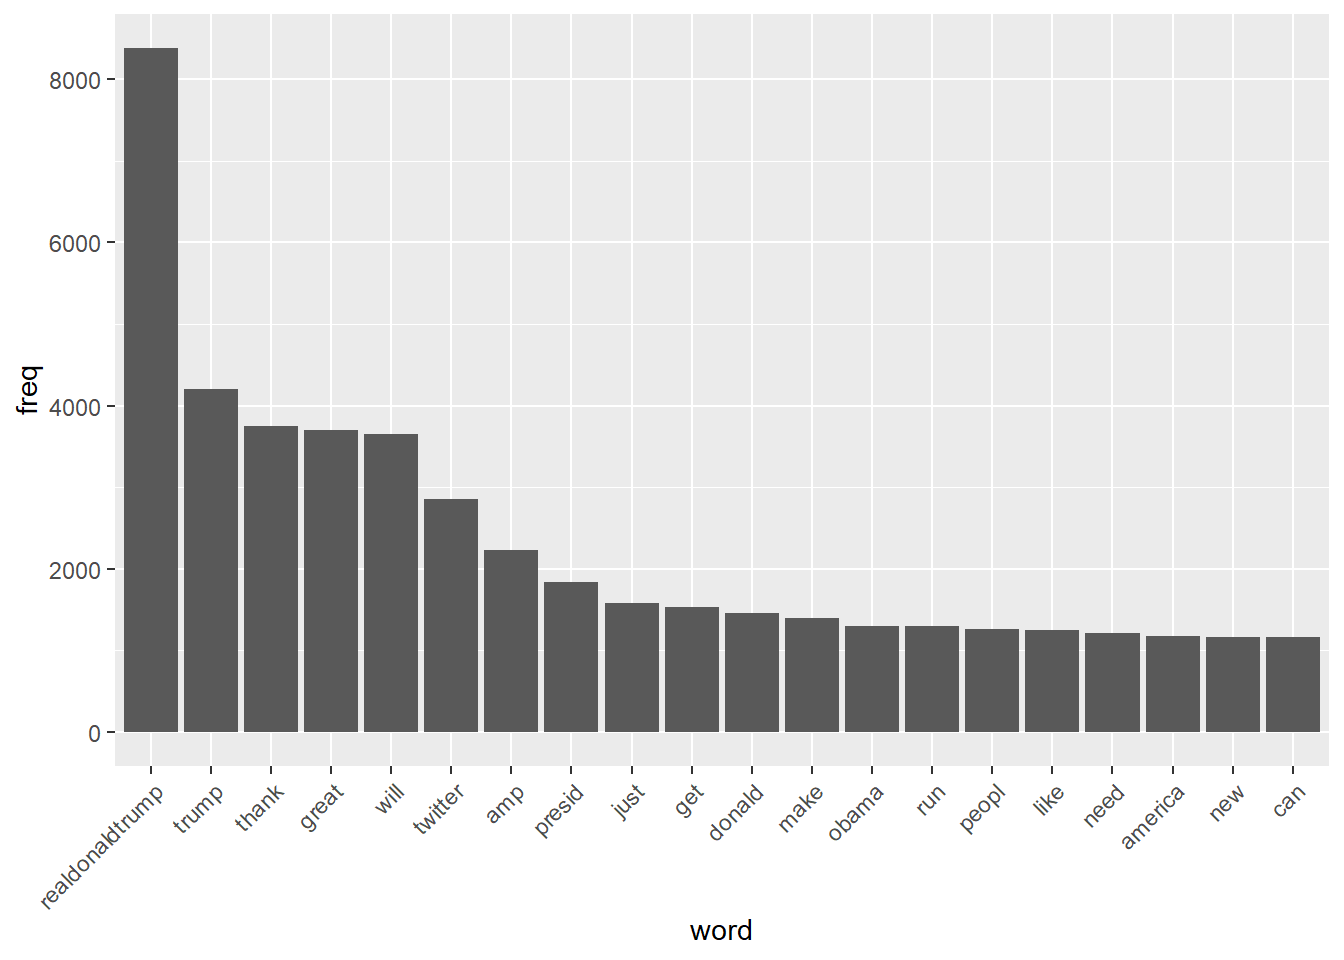
\includegraphics{HW2_files/figure-latex/unnamed-chunk-4-1.pdf}

\begin{Shaded}
\begin{Highlighting}[]
\NormalTok{tidy_dtm_post }\OperatorTok\StringTok{ }\KeywordTok{group_by}\NormalTok{(term) }\OperatorTok
\StringTok{  }\KeywordTok{summarize}\NormalTok{(}\DataTypeTok{freq =} \KeywordTok{sum}\NormalTok{(count)) }\OperatorTok
\StringTok{  }\KeywordTok{top_n}\NormalTok{(}\DecValTok{20}\NormalTok{, freq) }\OperatorTok
\StringTok{  }\KeywordTok{arrange}\NormalTok{(}\KeywordTok{desc}\NormalTok{(freq))}
\end{Highlighting}
\end{Shaded}

\begin{verbatim}
## # A tibble: 20 x 2
##    term      freq
##    <chr>    <dbl>
##  1 will       576
##  2 great      564
##  3 amp        497
##  4 peopl      231
##  5 news       225
##  6 thank      222
##  7 job        202
##  8 fake       194
##  9 tax        194
## 10 just       191
## 11 today      186
## 12 america    184
## 13 big        181
## 14 presid     179
## 15 countri    175
## 16 now        172
## 17 american   170
## 18 get        167
## 19 year       163
## 20 trump      160
\end{verbatim}

\begin{Shaded}
\begin{Highlighting}[]
\NormalTok{tidy_dtm_post }\OperatorTok\StringTok{ }\KeywordTok{group_by}\NormalTok{(term) }\OperatorTok
\StringTok{  }\KeywordTok{summarize}\NormalTok{(}\DataTypeTok{freq =} \KeywordTok{sum}\NormalTok{(count)) }\OperatorTok
\StringTok{  }\KeywordTok{top_n}\NormalTok{(}\DecValTok{20}\NormalTok{, freq) }\OperatorTok
\StringTok{  }\KeywordTok{arrange}\NormalTok{(}\KeywordTok{desc}\NormalTok{(freq)) }\OperatorTok
\StringTok{  }\KeywordTok{ggplot}\NormalTok{(}\KeywordTok{aes}\NormalTok{(}\KeywordTok{reorder}\NormalTok{(term, }\OperatorTok{-}\NormalTok{freq), freq)) }\OperatorTok{+}
\StringTok{  }\KeywordTok{geom_bar}\NormalTok{(}\DataTypeTok{stat=}\StringTok{"identity"}\NormalTok{) }\OperatorTok{+}
\StringTok{  }\KeywordTok{theme}\NormalTok{(}\DataTypeTok{axis.text.x =} \KeywordTok{element_text}\NormalTok{(}\DataTypeTok{angle=}\DecValTok{45}\NormalTok{, }\DataTypeTok{hjust=}\DecValTok{1}\NormalTok{)) }\OperatorTok{+}
\StringTok{  }\KeywordTok{xlab}\NormalTok{(}\StringTok{"word"}\NormalTok{)}
\end{Highlighting}
\end{Shaded}

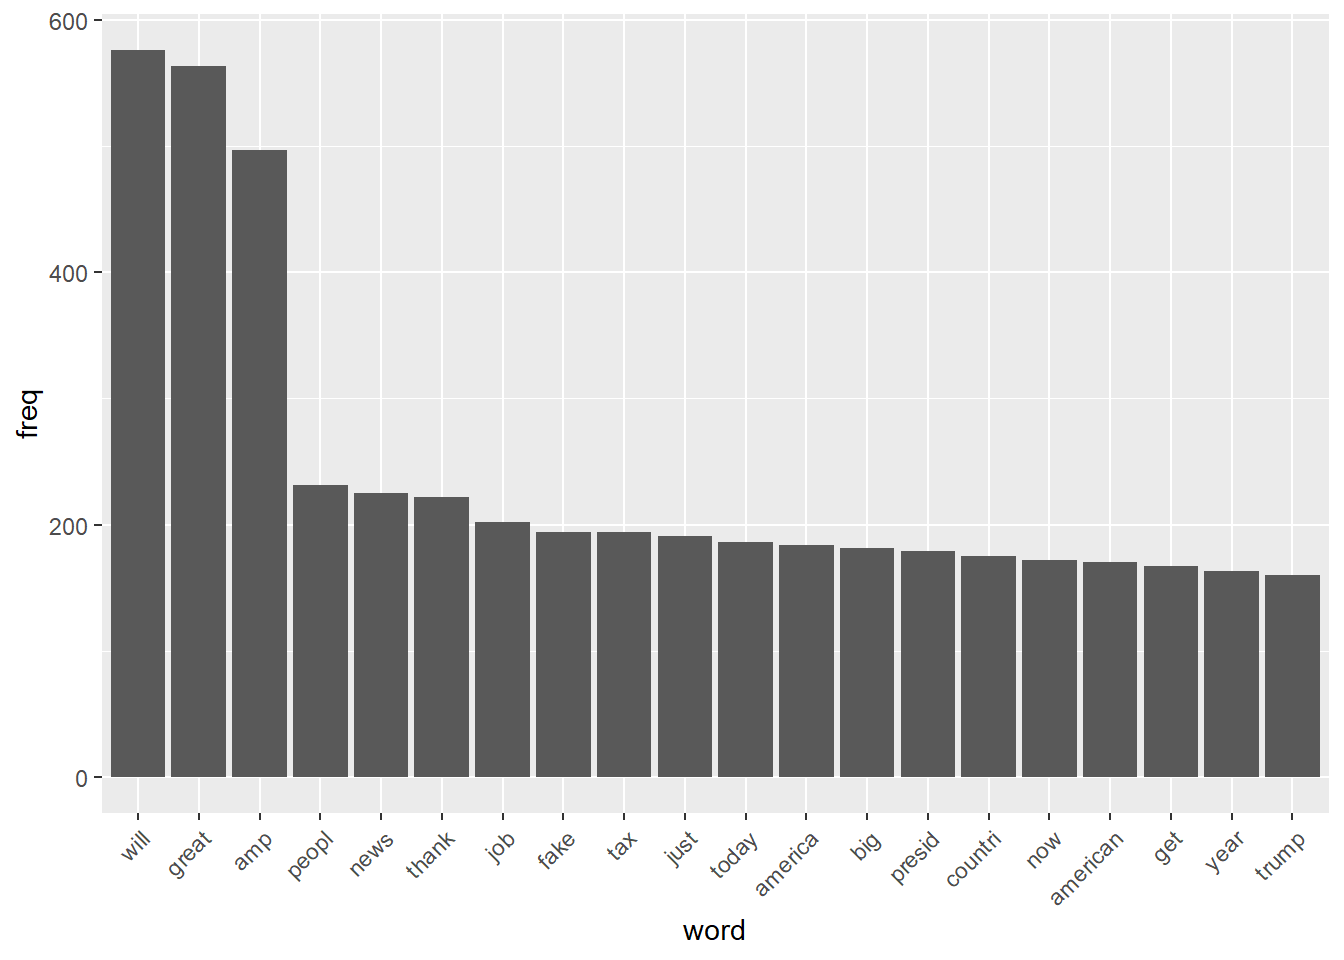
\includegraphics{HW2_files/figure-latex/unnamed-chunk-4-2.pdf} Prior to
the election, the top words used in the tweets revolved around
realdonaldtrump, trump, thank, great, will. These words occured with the
highest frequency. After the election, the words with the highest
frequency are will, great, amp. We note that prior to the election,
Trump uses words that promises certain goals, such as ``will'' and
``great''. He also asserts his brand by tweeting trump and
realdonaldtrump frequently. After the election, Trump started using less
words to assert his brand, presumably because he already has
recognition. Instead, Trump used more words to describe his policies,
such as ``tax''.

\subsubsection{(c) + (d) + (e)}\label{c-d-e}

\begin{Shaded}
\begin{Highlighting}[]
\NormalTok{removeMostPunctuation<-}
\ControlFlowTok{function}\NormalTok{ (x, }\DataTypeTok{preserve_intra_word_dashes =} \OtherTok{FALSE}\NormalTok{) }
\NormalTok{\{}
\NormalTok{    rmpunct <-}\StringTok{ }\ControlFlowTok{function}\NormalTok{(x) \{}
\NormalTok{        x <-}\StringTok{ }\KeywordTok{gsub}\NormalTok{(}\StringTok{"#"}\NormalTok{, }\StringTok{"}\CharTok{\textbackslash{}002}\StringTok{"}\NormalTok{, x)}
\NormalTok{        x <-}\StringTok{ }\KeywordTok{gsub}\NormalTok{(}\StringTok{"[[:punct:]]+"}\NormalTok{, }\StringTok{""}\NormalTok{, x)}
        \KeywordTok{gsub}\NormalTok{(}\StringTok{"}\CharTok{\textbackslash{}002}\StringTok{"}\NormalTok{, }\StringTok{"#"}\NormalTok{, x, }\DataTypeTok{fixed =} \OtherTok{TRUE}\NormalTok{)}
\NormalTok{    \}}
    \ControlFlowTok{if}\NormalTok{ (preserve_intra_word_dashes) \{ }
\NormalTok{        x <-}\StringTok{ }\KeywordTok{gsub}\NormalTok{(}\StringTok{"(}\CharTok{\textbackslash{}\textbackslash{}}\StringTok{w)-(}\CharTok{\textbackslash{}\textbackslash{}}\StringTok{w)"}\NormalTok{, }\StringTok{"}\CharTok{\textbackslash{}\textbackslash{}}\StringTok{1}\CharTok{\textbackslash{}001\textbackslash{}\textbackslash{}}\StringTok{2"}\NormalTok{, x)}
\NormalTok{        x <-}\StringTok{ }\KeywordTok{rmpunct}\NormalTok{(x)}
        \KeywordTok{gsub}\NormalTok{(}\StringTok{"}\CharTok{\textbackslash{}001}\StringTok{"}\NormalTok{, }\StringTok{"-"}\NormalTok{, x, }\DataTypeTok{fixed =} \OtherTok{TRUE}\NormalTok{)}
\NormalTok{    \} }\ControlFlowTok{else}\NormalTok{ \{}
        \KeywordTok{rmpunct}\NormalTok{(x)}
\NormalTok{    \}}
\NormalTok{\}}

\NormalTok{trumptweets_hashtags <-}\StringTok{ }\KeywordTok{Corpus}\NormalTok{(}\KeywordTok{VectorSource}\NormalTok{(tweets}\OperatorTok{$}\NormalTok{text))}
\NormalTok{trumptweets_hashtags <-}\StringTok{ }\KeywordTok{tm_map}\NormalTok{(trumptweets_hashtags, tolower)}
\end{Highlighting}
\end{Shaded}

\begin{verbatim}
## Warning in tm_map.SimpleCorpus(trumptweets_hashtags, tolower):
## transformation drops documents
\end{verbatim}

\begin{Shaded}
\begin{Highlighting}[]
\NormalTok{trumptweets_hashtags <-}\StringTok{ }\KeywordTok{tm_map}\NormalTok{(trumptweets_hashtags, removeWords, }\KeywordTok{stopwords}\NormalTok{(}\StringTok{"en"}\NormalTok{))}
\end{Highlighting}
\end{Shaded}

\begin{verbatim}
## Warning in tm_map.SimpleCorpus(trumptweets_hashtags, removeWords,
## stopwords("en")): transformation drops documents
\end{verbatim}

\begin{Shaded}
\begin{Highlighting}[]
\NormalTok{trumptweets_hashtags <-}\StringTok{ }\KeywordTok{tm_map}\NormalTok{(trumptweets_hashtags, }\KeywordTok{content_transformer}\NormalTok{(removeMostPunctuation),}
    \DataTypeTok{preserve_intra_word_dashes =} \OtherTok{TRUE}\NormalTok{)}
\end{Highlighting}
\end{Shaded}

\begin{verbatim}
## Warning in tm_map.SimpleCorpus(trumptweets_hashtags,
## content_transformer(removeMostPunctuation), : transformation drops
## documents
\end{verbatim}

\begin{Shaded}
\begin{Highlighting}[]
\NormalTok{trumptweets_hashtags <-}\StringTok{ }\KeywordTok{tm_map}\NormalTok{(trumptweets_hashtags,stemDocument)}
\end{Highlighting}
\end{Shaded}

\begin{verbatim}
## Warning in tm_map.SimpleCorpus(trumptweets_hashtags, stemDocument):
## transformation drops documents
\end{verbatim}

\begin{Shaded}
\begin{Highlighting}[]
\NormalTok{dtm_hashtags <-}\StringTok{ }\KeywordTok{DocumentTermMatrix}\NormalTok{(trumptweets_hashtags)}
\NormalTok{dtm_hashtags <-}\StringTok{ }\KeywordTok{removeSparseTerms}\NormalTok{(dtm_hashtags,.}\DecValTok{99}\NormalTok{)}
\NormalTok{tidy_dtm_hashtags <-}\StringTok{ }\KeywordTok{tidy}\NormalTok{(dtm_hashtags)}
\NormalTok{dtm.mat.hashtags <-}\StringTok{ }\KeywordTok{as.matrix}\NormalTok{(dtm_hashtags)}
\NormalTok{tidy_dtm_hashtags_filt <-}\StringTok{ }\KeywordTok{filter}\NormalTok{(tidy_dtm_hashtags, }\KeywordTok{grepl}\NormalTok{(}\StringTok{"^#.*"}\NormalTok{, tidy_dtm_hashtags}\OperatorTok{$}\NormalTok{term))}

\NormalTok{tidy_dtm_hashtags_filt }\OperatorTok\StringTok{ }\KeywordTok{group_by}\NormalTok{(term) }\OperatorTok\StringTok{ }
\StringTok{  }\KeywordTok{summarize}\NormalTok{(}\DataTypeTok{freq =} \KeywordTok{sum}\NormalTok{(count)) }\OperatorTok
\StringTok{  }\KeywordTok{top_n}\NormalTok{(}\DecValTok{5}\NormalTok{, freq) }\OperatorTok
\StringTok{  }\KeywordTok{arrange}\NormalTok{(}\KeywordTok{desc}\NormalTok{(freq)) }\OperatorTok
\StringTok{  }\KeywordTok{ggplot}\NormalTok{(}\KeywordTok{aes}\NormalTok{(}\KeywordTok{reorder}\NormalTok{(term, }\OperatorTok{-}\NormalTok{freq), freq)) }\OperatorTok{+}
\StringTok{  }\KeywordTok{geom_bar}\NormalTok{(}\DataTypeTok{stat=}\StringTok{"identity"}\NormalTok{) }\OperatorTok{+}
\StringTok{  }\KeywordTok{theme}\NormalTok{(}\DataTypeTok{axis.text.x =} \KeywordTok{element_text}\NormalTok{(}\DataTypeTok{angle=}\DecValTok{45}\NormalTok{, }\DataTypeTok{hjust=}\DecValTok{1}\NormalTok{)) }\OperatorTok{+}
\StringTok{  }\KeywordTok{xlab}\NormalTok{(}\StringTok{"word"}\NormalTok{)}
\end{Highlighting}
\end{Shaded}

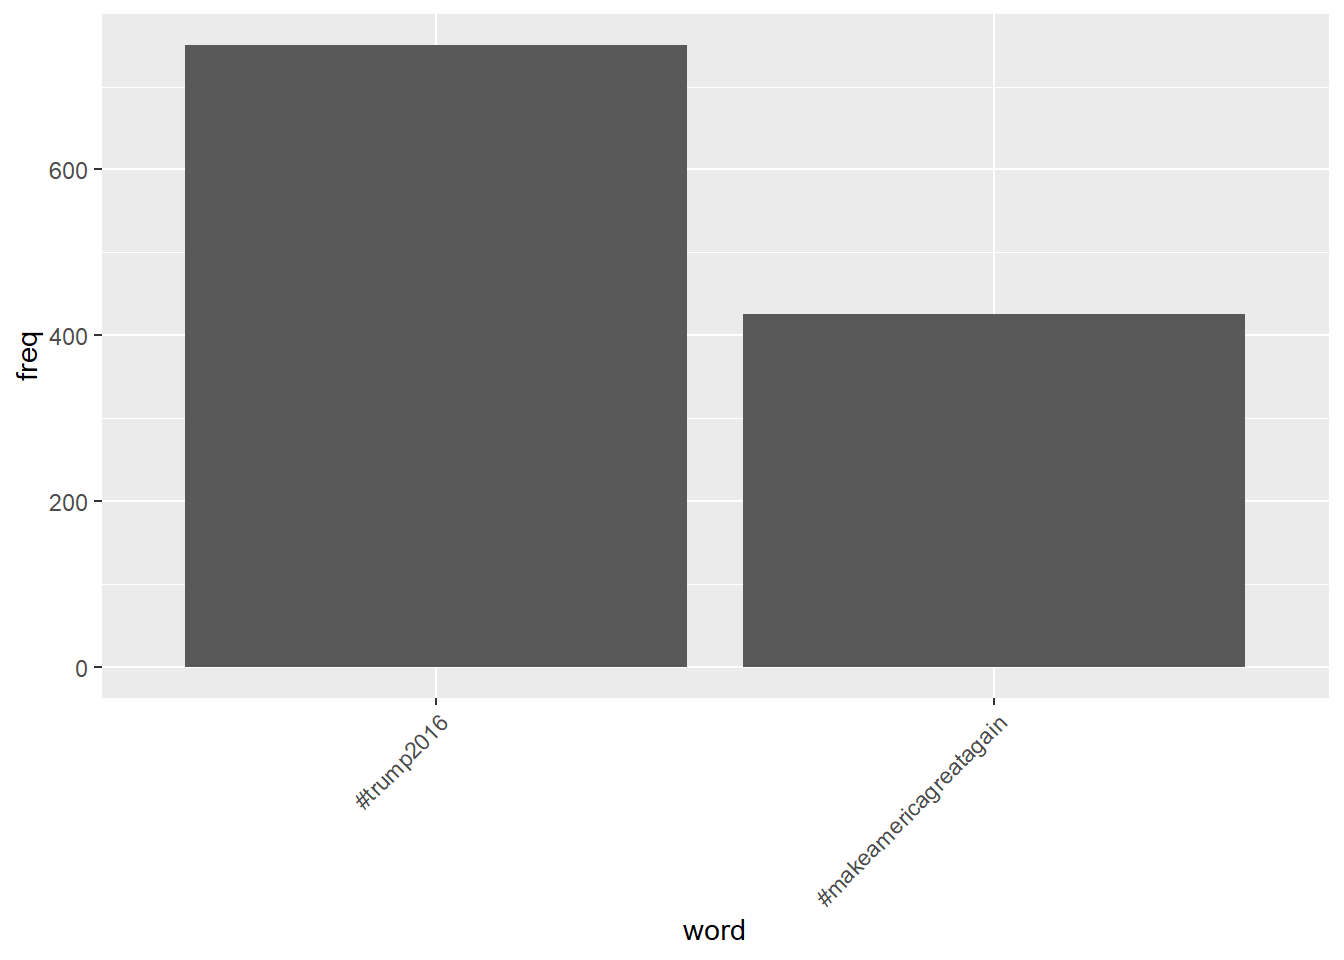
\includegraphics{HW2_files/figure-latex/unnamed-chunk-5-1.pdf}

\subsubsection{(f)}\label{f}

\begin{Shaded}
\begin{Highlighting}[]
\NormalTok{bigram.docs <-}\StringTok{ }\NormalTok{tweets }\OperatorTok\StringTok{ }
\KeywordTok{unnest_tokens}\NormalTok{(bigram, text, }\DataTypeTok{token =} \StringTok{"ngrams"}\NormalTok{, }\DataTypeTok{n =} \DecValTok{2}\NormalTok{)}
\NormalTok{bigram.docs <-}\StringTok{ }\KeywordTok{filter}\NormalTok{(bigram.docs, bigram }\OperatorTok{==}\StringTok{ "crooked hillary"}\NormalTok{)}
\NormalTok{bigram.docs <-}\StringTok{ }\KeywordTok{mutate}\NormalTok{(bigram.docs, }\DataTypeTok{created_at =} \KeywordTok{mdy_hms}\NormalTok{(created_at))}
\end{Highlighting}
\end{Shaded}

\begin{verbatim}
## Warning: All formats failed to parse. No formats found.
\end{verbatim}

\begin{Shaded}
\begin{Highlighting}[]
\NormalTok{bigram.docs <-}\StringTok{ }\KeywordTok{mutate}\NormalTok{(bigram.docs, }\DataTypeTok{n =} \DecValTok{1}\NormalTok{)}
\NormalTok{bigram.docs }\OperatorTok\StringTok{ }
\StringTok{  }\KeywordTok{group_by}\NormalTok{(}\DataTypeTok{month=}\KeywordTok{format}\NormalTok{(}\KeywordTok{as.Date}\NormalTok{(created_at),}\DataTypeTok{format=}\StringTok{"%m"}\NormalTok{)) }\OperatorTok\StringTok{ }\KeywordTok{summarize}\NormalTok{(}\DataTypeTok{freq=}\KeywordTok{sum}\NormalTok{(n)) }\OperatorTok
\StringTok{  }\KeywordTok{ungroup}\NormalTok{() ->}\StringTok{ }\NormalTok{df2}
\NormalTok{df2}
\end{Highlighting}
\end{Shaded}

\begin{verbatim}
## # A tibble: 1 x 2
##   month  freq
##   <chr> <dbl>
## 1 <NA>    227
\end{verbatim}


\end{document}
